\reportchapter{1}{Contexte G\'{e}n\'{e}ral, \'{E}tude de l'Existant et Gestion de Projet}{Pr\'{e}sentation institutionnelle de PortNet S.A., organigramme, partenariat douanier ADII/BADR, \'{e}tude et critique de l'existant, cahier des charges fonctionnel et non-fonctionnel, choix de la stack technologique et m\'{e}thodologie Agile/Scrum.}

\section*{Introduction}

Ce premier chapitre pose le cadre institutionnel, m\'{e}tier et m\'{e}thodologique dans lequel s'inscrit le pr\'{e}sent Projet de Fin d'Ann\'{e}e. Il pr\'{e}sente successivement l'organisme d'accueil PortNet S.A., son r\^{o}le strat\'{e}gique de Guichet Unique National et son organigramme fonctionnel. Il examine ensuite le partenariat critique avec l'Administration des Douanes et Imp\^{o}ts Indirects (ADII) et son syst\`{e}me BADR. Apr\`{e}s une \'{e}tude approfondie et une critique argument\'{e}e du processus manuel existant, le chapitre formalise la probl\'{e}matique m\'{e}tier, les verrous techniques identifi\'{e}s, le cahier des charges fonctionnel et non-fonctionnel, le choix de la stack technologique et, enfin, la d\'{e}marche de conduite de projet Agile Scrum adopt\'{e}e.

\section{L'organisme d'accueil}

\textbf{PortNet S.A.} est une entreprise initiée en 2008 par l'Agence Nationale
des Ports (l'autorité portuaire au Maroc). Elle est le fruit de l'alliance
stratégique des communautés portuaires et du commerce international. Il s'agit
d'un outil propre au gouvernement marocain visant la mise en \oe uvre de
plusieurs stratégies sectorielles en vue de l'amélioration du climat des
affaires, des échanges commerciaux, de la compétitivité portuaire et logistique
et de leur généralisation, sans oublier pour autant l'innovation dans les
services e-gov.

Concrètement, PortNet opère le \textbf{Guichet Unique National des procédures du
commerce extérieur} : une plateforme électronique communautaire qui dématérialise
et centralise l'ensemble des formalités liées aux opérations d'importation,
d'exportation et de logistique portuaire, en interconnectant en un point d'entrée
unique les administrations, les organismes de contrôle, les opérateurs
portuaires, les banques et les entreprises importatrices et exportatrices.

\begin{figure}[H]
  \centering
  
\includegraphics[width=5cm]{Logos/portnet_logo_cropped.png}
  \caption{Logo de PortNet S.A.}
  \label{fig:logo-portnet}
\end{figure}

\subsection{Données clés}

Actuellement, PortNet a franchi la barre des \textbf{66 000 usagers}, incluant
plus de 55 000 importateurs et exportateurs, 1 700 déclarants et transitaires, 20
banques et 43 administrations. La plateforme fédère également 200 agents
maritimes et consignataires, plus de 300 \textit{freight forwarders}, 43
opérateurs de manutention, 62 opérateurs MEAD et 5 expressistes, répartis sur 12
ports et 11 aéroports. Elle met à disposition plus de \textbf{120 services en
ligne} et a acheminé plus de 136 millions de messages EDI.

\begin{figure}[H]
  \centering
  \includegraphics[width=0.85\textwidth]{images/portnet-chiffres.jpg}
  \caption{PortNet en chiffres}
  \label{fig:portnet-chiffres}
\end{figure}

\subsection{L'organigramme de PortNet S.A.}

\begin{figure}[H]
  \centering
  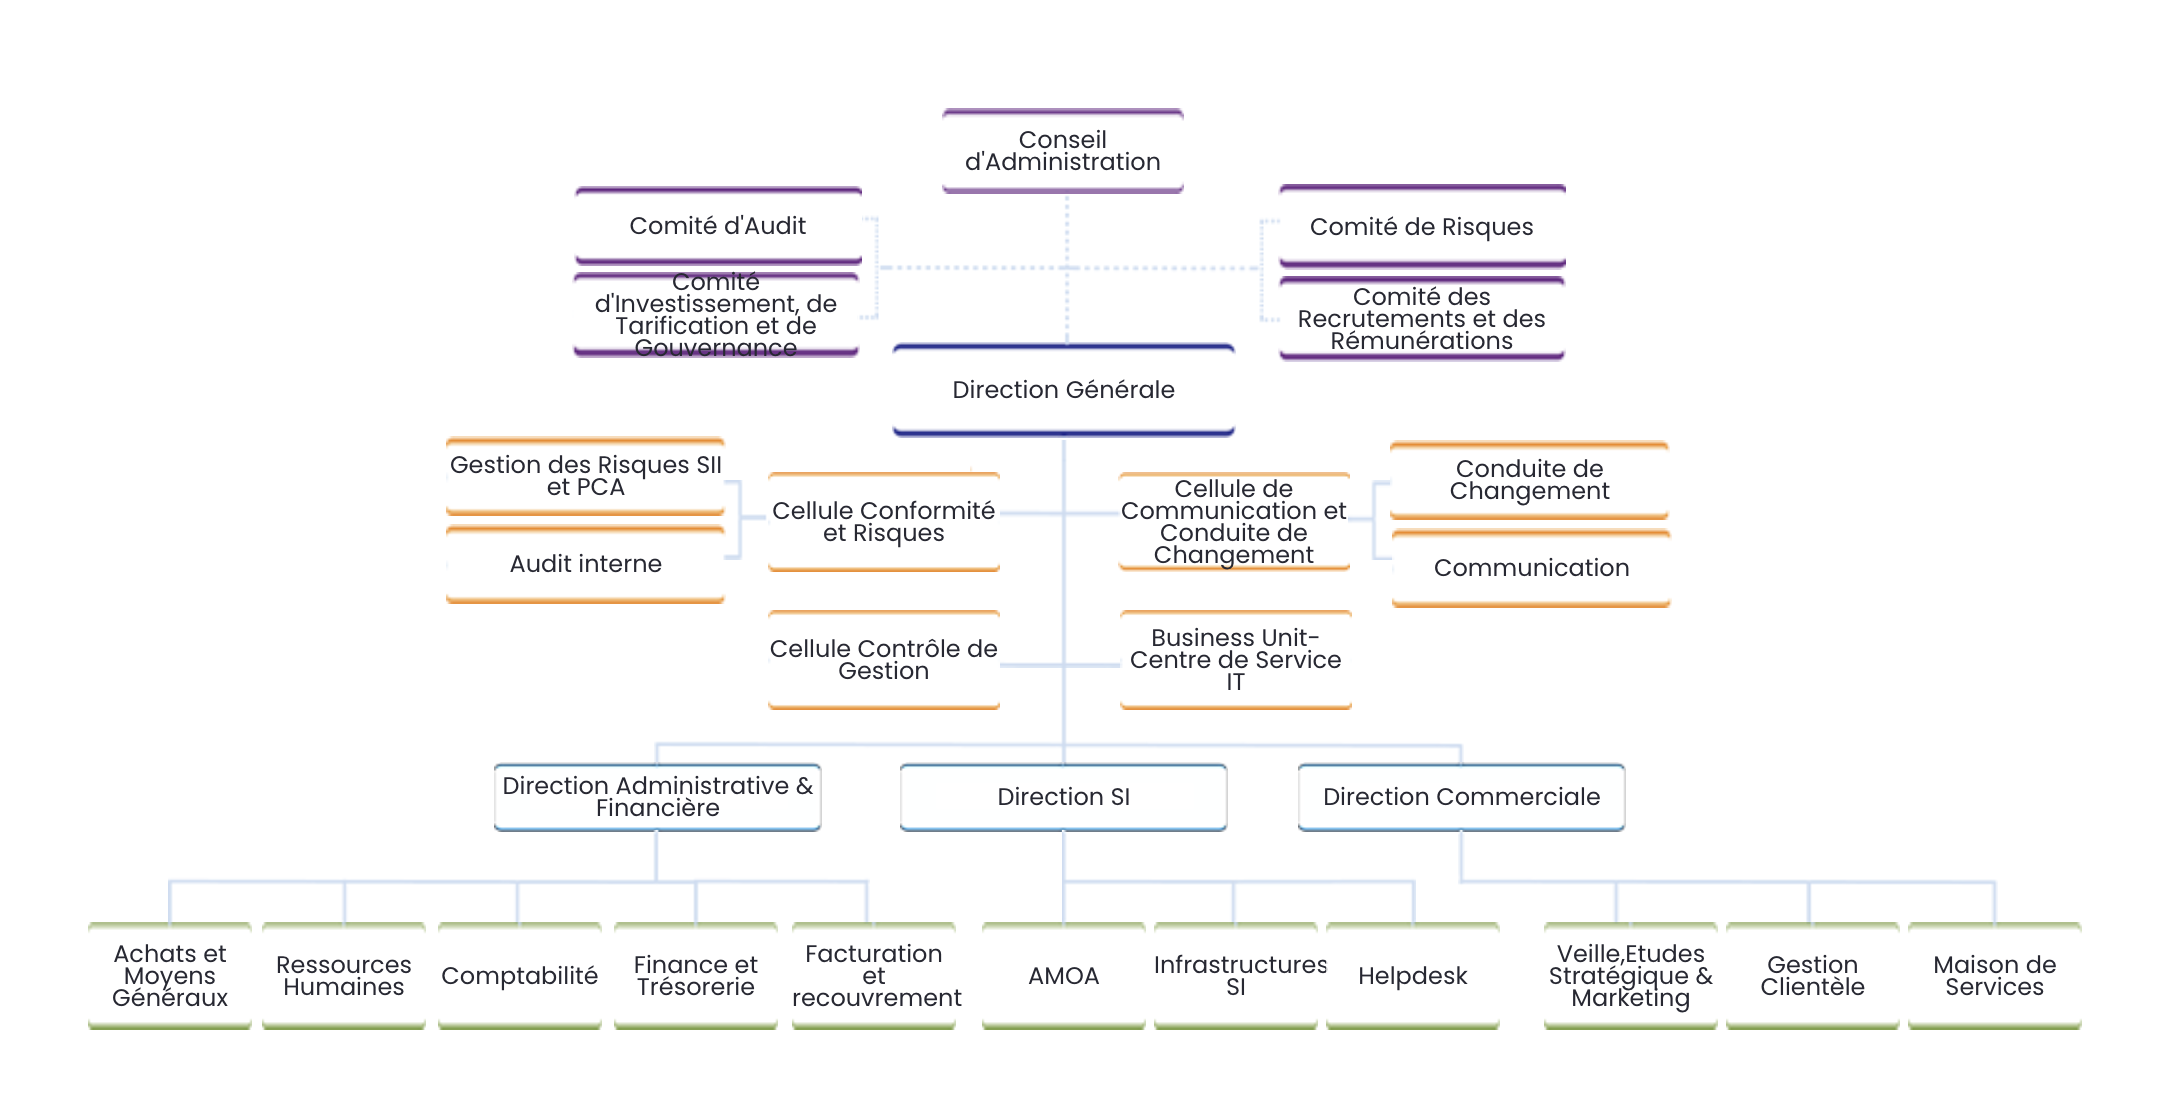
\includegraphics[width=\textwidth]{images/portnet_organisme.png}
  \caption{L'organigramme de PortNet S.A.}
  \label{fig:organigramme}
\end{figure}

L'organigramme de PortNet montre que l'entreprise est dirigée par
\textbf{M. Youssef AHOUZI}, Directeur Général. L'organisation comprend plusieurs
comités, notamment le Conseil d'Administration, le Comité d'Audit, le Comité
d'Investissement, de Tarification et de Gouvernance, le Comité de Risques et le
Comité des Recrutements et des Rémunérations.

La Direction Générale s'appuie sur des cellules transverses --- Conformité et
Risques, Communication et Conduite de Changement, Contrôle de Gestion, Gestion
des Risques SI et Plan de Continuité d'Activité, Audit interne --- ainsi que sur
une \textit{Business Unit} Centre de Service IT. Trois directions opérationnelles
structurent l'activité :

\begin{itemize}[leftmargin=1.6cm,itemsep=2pt,topsep=4pt]
  \item la \textbf{Direction Administrative \& Financière} (achats et moyens
        généraux, ressources humaines, comptabilité, finance et trésorerie,
        facturation et recouvrement) ;
  \item la \textbf{Direction SI} (AMOA, infrastructures SI, \textit{helpdesk}) ;
  \item la \textbf{Direction Commerciale} (veille et études stratégiques,
        marketing, gestion clientèle, maison de services).
\end{itemize}

Mon stage s'est déroulé au sein de la \textbf{Direction SI}, en interaction
directe avec les équipes fonctionnelles responsables du processus de souscription.

\subsection{Les services de l'entreprise}

PortNet met à disposition de sa communauté plus de 120 services en ligne. Parmi
les principaux :

\begin{itemize}[leftmargin=1.6cm,itemsep=3pt,topsep=4pt]
  \item \textbf{Souscription en ligne} : inscription dématérialisée des opérateurs
        économiques à la plateforme et, le cas échéant, auprès de l'administration
        des douanes. C'est le service directement concerné par le présent projet ;
  \item \textbf{Trade Direct} : gestion en ligne des opérations d'import et
        d'export (titres, engagements d'importation, licences) ;
  \item \textbf{Trade Sense} : services d'information et d'aide à la décision sur
        les procédures et les flux du commerce extérieur ;
  \item \textbf{Massar Attajir} : suivi et traçabilité du parcours de l'opération
        commerciale ;
  \item \textbf{Gestion des accès portuaires} : badges, autorisations et contrôle
        d'accès aux enceintes portuaires.
\end{itemize}

\section{\'{E}tude et Critique de l'Existant}

\subsection{Description du Processus Actuel de Souscription}

Le processus d'abonnement aux services PortNet exige la fourniture et la v\'{e}rification de neuf pi\`{e}ces justificatives r\'{e}glementaires :

\begin{enumerate}[leftmargin=*, itemsep=4pt]
    \item Le \textbf{Mod\`{e}le J} (Extrait du Registre de Commerce d\'{e}livr\'{e} par le Greffe du Tribunal de Commerce) ;
    \item Le \textbf{Bulletin de Notification de l'Identifiant Fiscal (IF)} (Mod\`{e}le DGI \texttt{AAC140B}) ;
    \item L'\textbf{Attestation d'Inscription \`{a} la Taxe Professionnelle (TP)} (Mod\`{e}le DGI \texttt{AAC060B}) ;
    \item Le \textbf{Certificat de l'Identifiant Commun de l'Entreprise (ICE)} (OMPIC/DGI) ;
    \item L'\textbf{Attestation de Domiciliation} (ou contrat de bail commercial, titre de propri\'{e}t\'{e}) ;
    \item L'\textbf{Attestation de Relev\'{e} d'Identit\'{e} Bancaire (RIB)} officielle ;
    \item La \textbf{Carte Nationale d'Identit\'{e} \'{E}lectronique (CNIE)} ou Passeport des g\'{e}rants ;
    \item Les \textbf{Statuts de la Soci\'{e}t\'{e}} ;
    \item La \textbf{Procuration} \'{e}ventuelle du repr\'{e}sentant l\'{e}gal.
\end{enumerate}

Dans l'existant, l'instruction des souscriptions repose enti\`{e}rement sur un contr\^{o}le visuel manuel r\'{e}alis\'{e} par des agents v\'{e}rificateurs. Chaque agent doit ouvrir chaque fichier PDF, lire les informations imprim\'{e}es, v\'{e}rifier visuellement la concordance des num\'{e}ros d'identification entre les diff\'{e}rents documents et comparer les donn\'{e}es avec le formulaire d'inscription rempli par l'op\'{e}rateur. Ce processus est d\'{e}taill\'{e} dans la figure~\ref{fig:processus-existant}.

\begin{figure}[H]
    \centering
    \IfFileExists{images/processus_souscription_existant.png}{\includegraphics[width=\textwidth]{images/processus_souscription_existant.png}}{\fbox{\parbox{14cm}{\centering\vspace{2cm}\textit{Processus actuel de souscription --- Exporter depuis processus\_souscription\_existant.drawio}\vspace{2cm}}}}
    \caption{Processus actuel de souscription et de v\'{e}rification manuelle des dossiers.}
    \label{fig:processus-existant}
\end{figure}

\subsection{R\'{e}f\'{e}rentiel Officiel et Guides Utilisateurs PortNet}

Pour concevoir et mod\'{e}liser la solution de v\'{e}rification documentaire automatique, une analyse approfondie du r\'{e}f\'{e}rentiel officiel de PortNet S.A. a \'{e}t\'{e} men\'{e}e. Le portail officiel des guides utilisateurs \cite{portnet-guides} (\url{https://www.portnet.ma/guides-utilisateurs}) met \`{a} disposition l'ensemble des manuels de proc\'{e}dure et r\'{e}glements m\'{e}tier de la plateforme.

\begin{figure}[H]
    \centering
    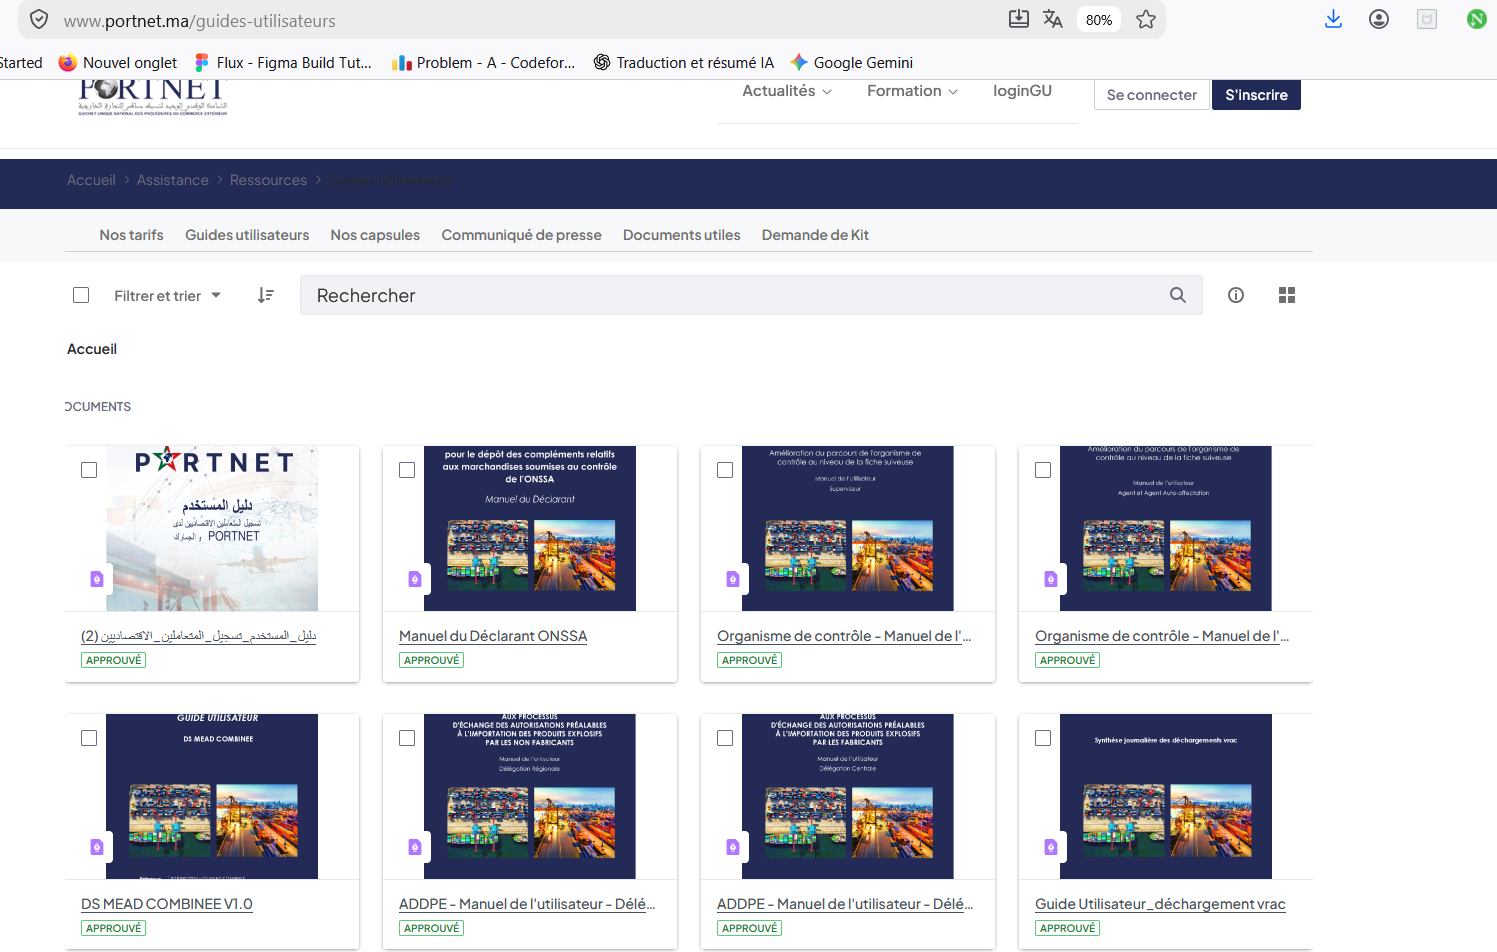
\includegraphics[width=0.88\textwidth]{images/portnet_portal_guides.png}
    \caption{Portail officiel des guides utilisateurs PortNet S.A. (\url{https://www.portnet.ma/guides-utilisateurs}).}
    \label{fig:portnet-portal-guides}
\end{figure}

Le document de r\'{e}f\'{e}rence principal utilis\'{e} tout au long du projet est le \textit{Guide Utilisateur --- Enregistrement des op\'{e}rateurs \'{e}conomiques aupr\`{e}s de PortNet et de la Douane} (\texttt{Gestion des souscriptions profil operateur economique.pdf}). Ce guide officiel d\'{e}taille la proc\'{e}dure d'inscription conjointe, le r\^{o}le des pi\`{e}ces justificatives et le circuit d'homologation des dossiers d'op\'{e}rateurs du commerce ext\'{e}rieur.

\begin{figure}[H]
    \centering
    \begin{minipage}[b]{0.48\textwidth}
        \centering
        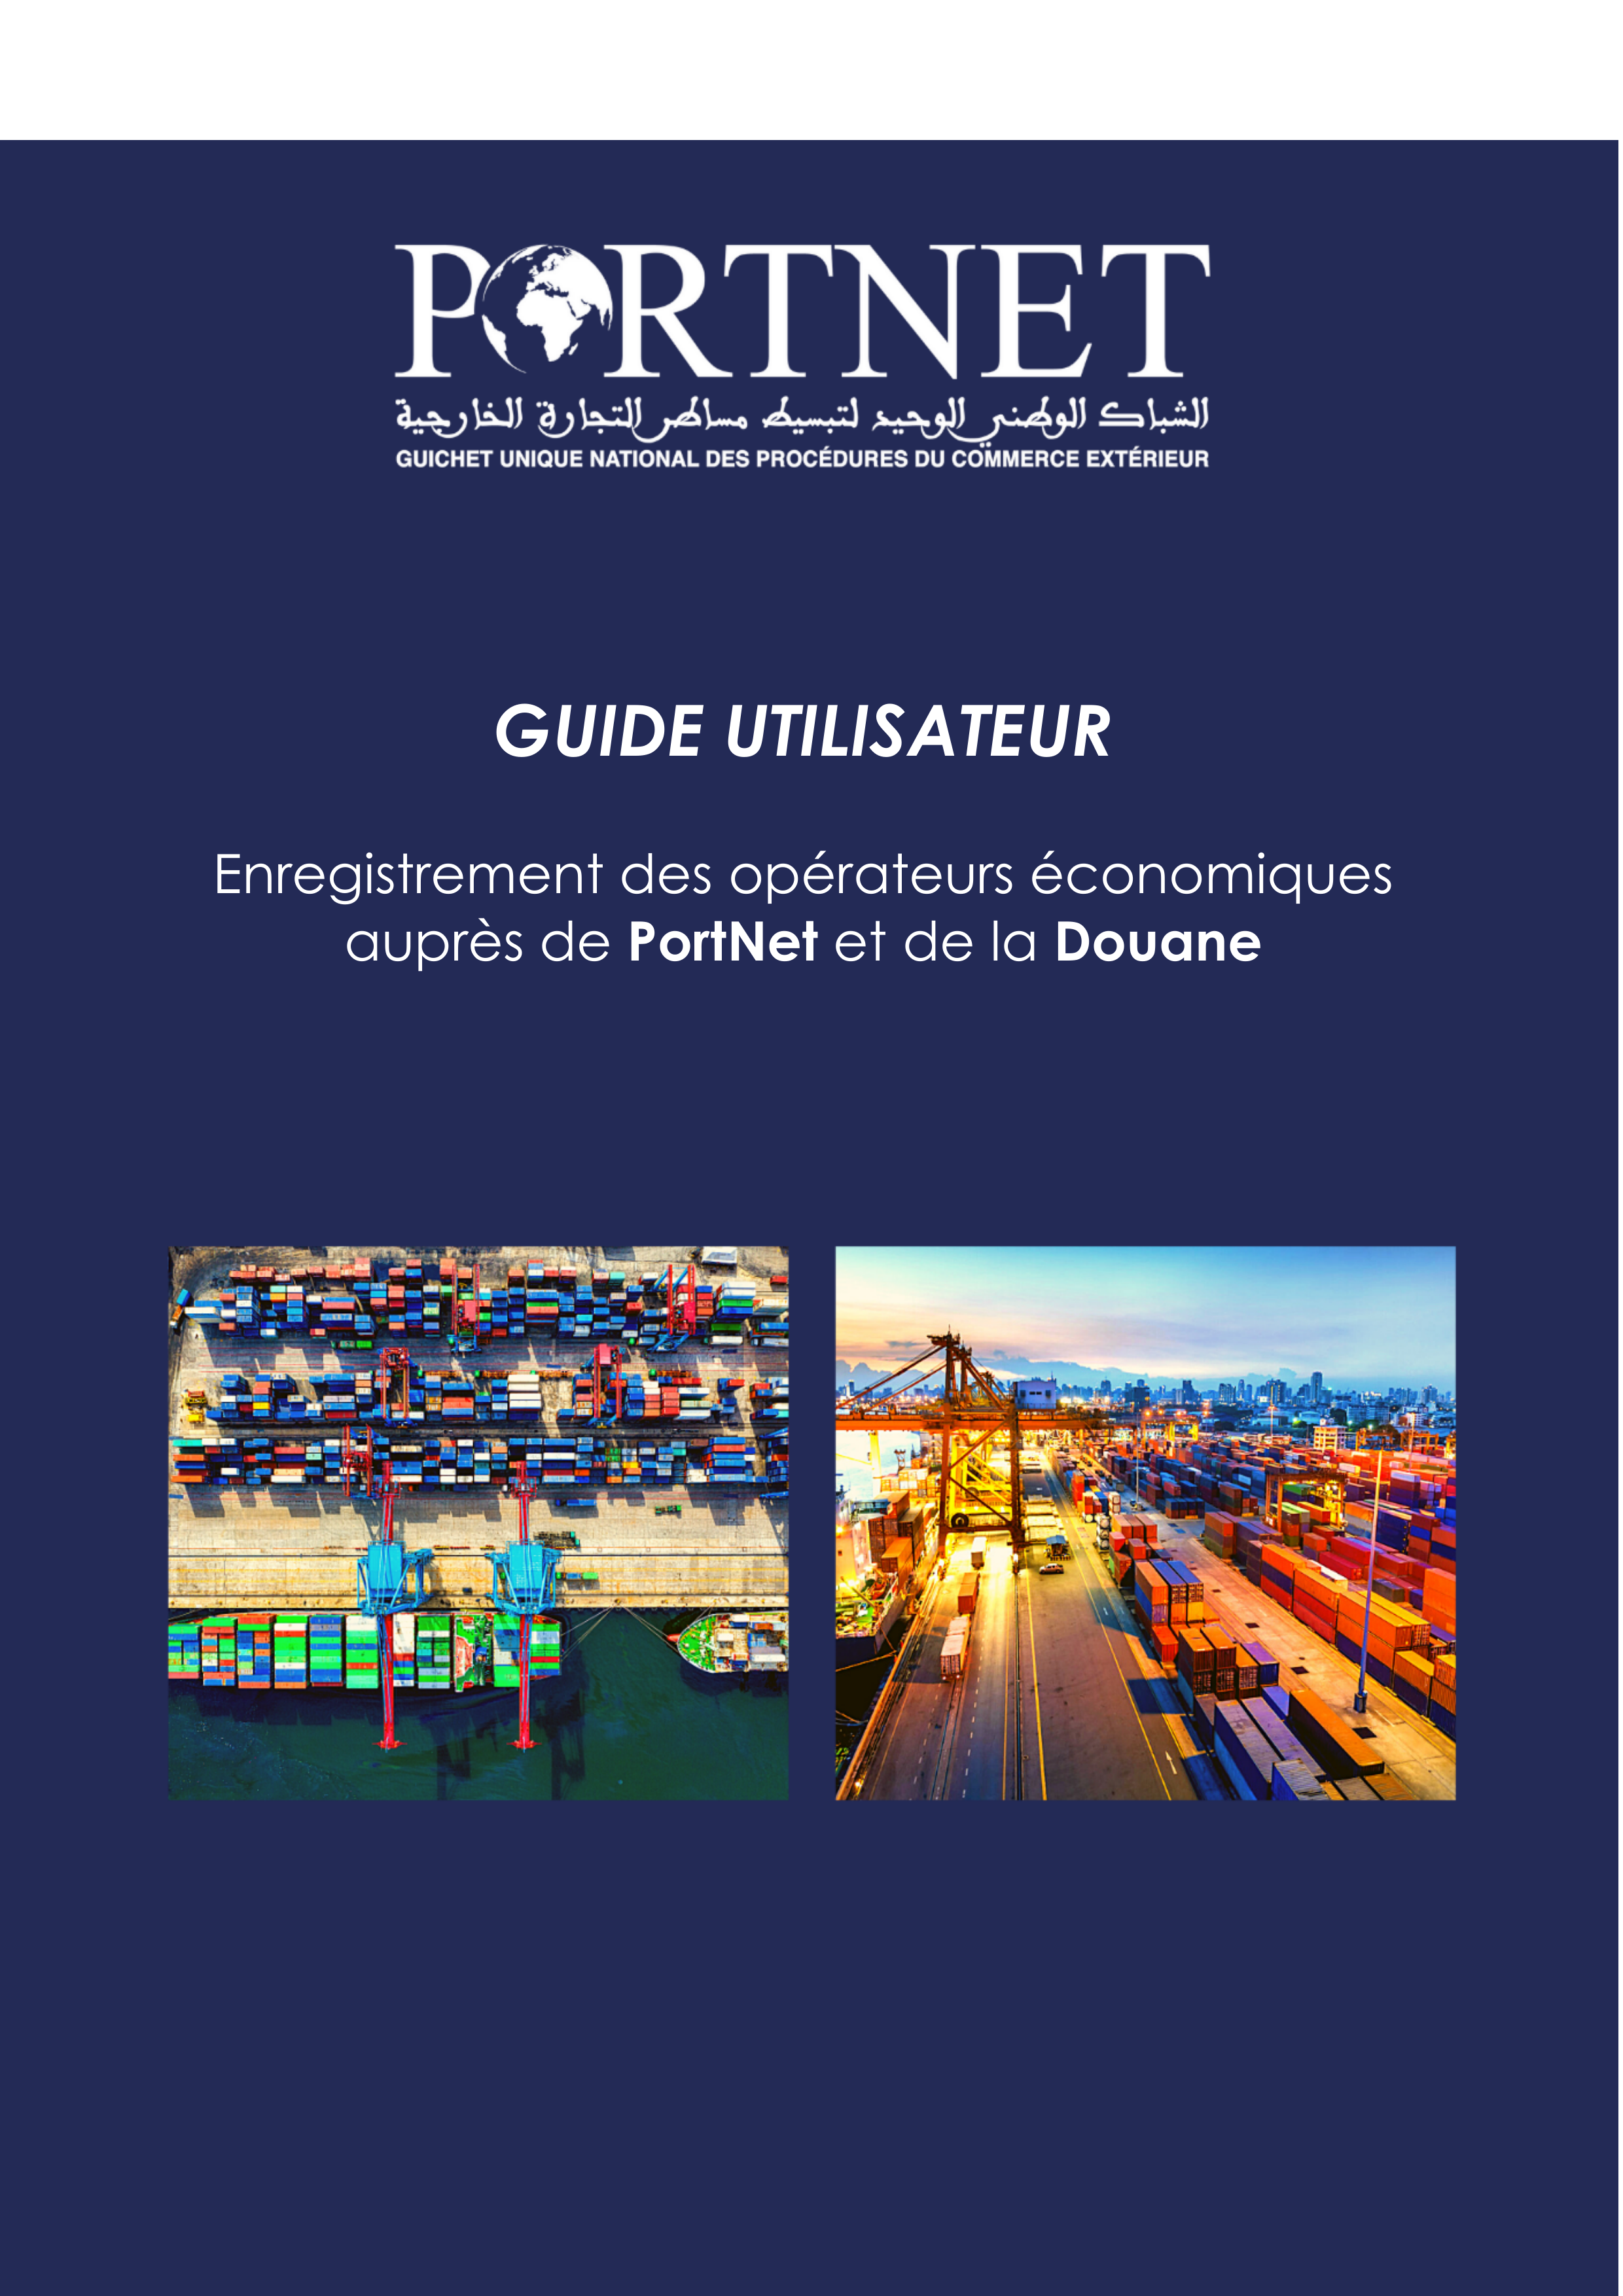
\includegraphics[width=\textwidth]{images/guide_utilisateur_couverture.png}
        \caption{Page de garde du Guide Utilisateur Officiel PortNet.}
        \label{fig:guide-couverture}
    \end{minipage}
    \hfill
    \begin{minipage}[b]{0.48\textwidth}
        \centering
        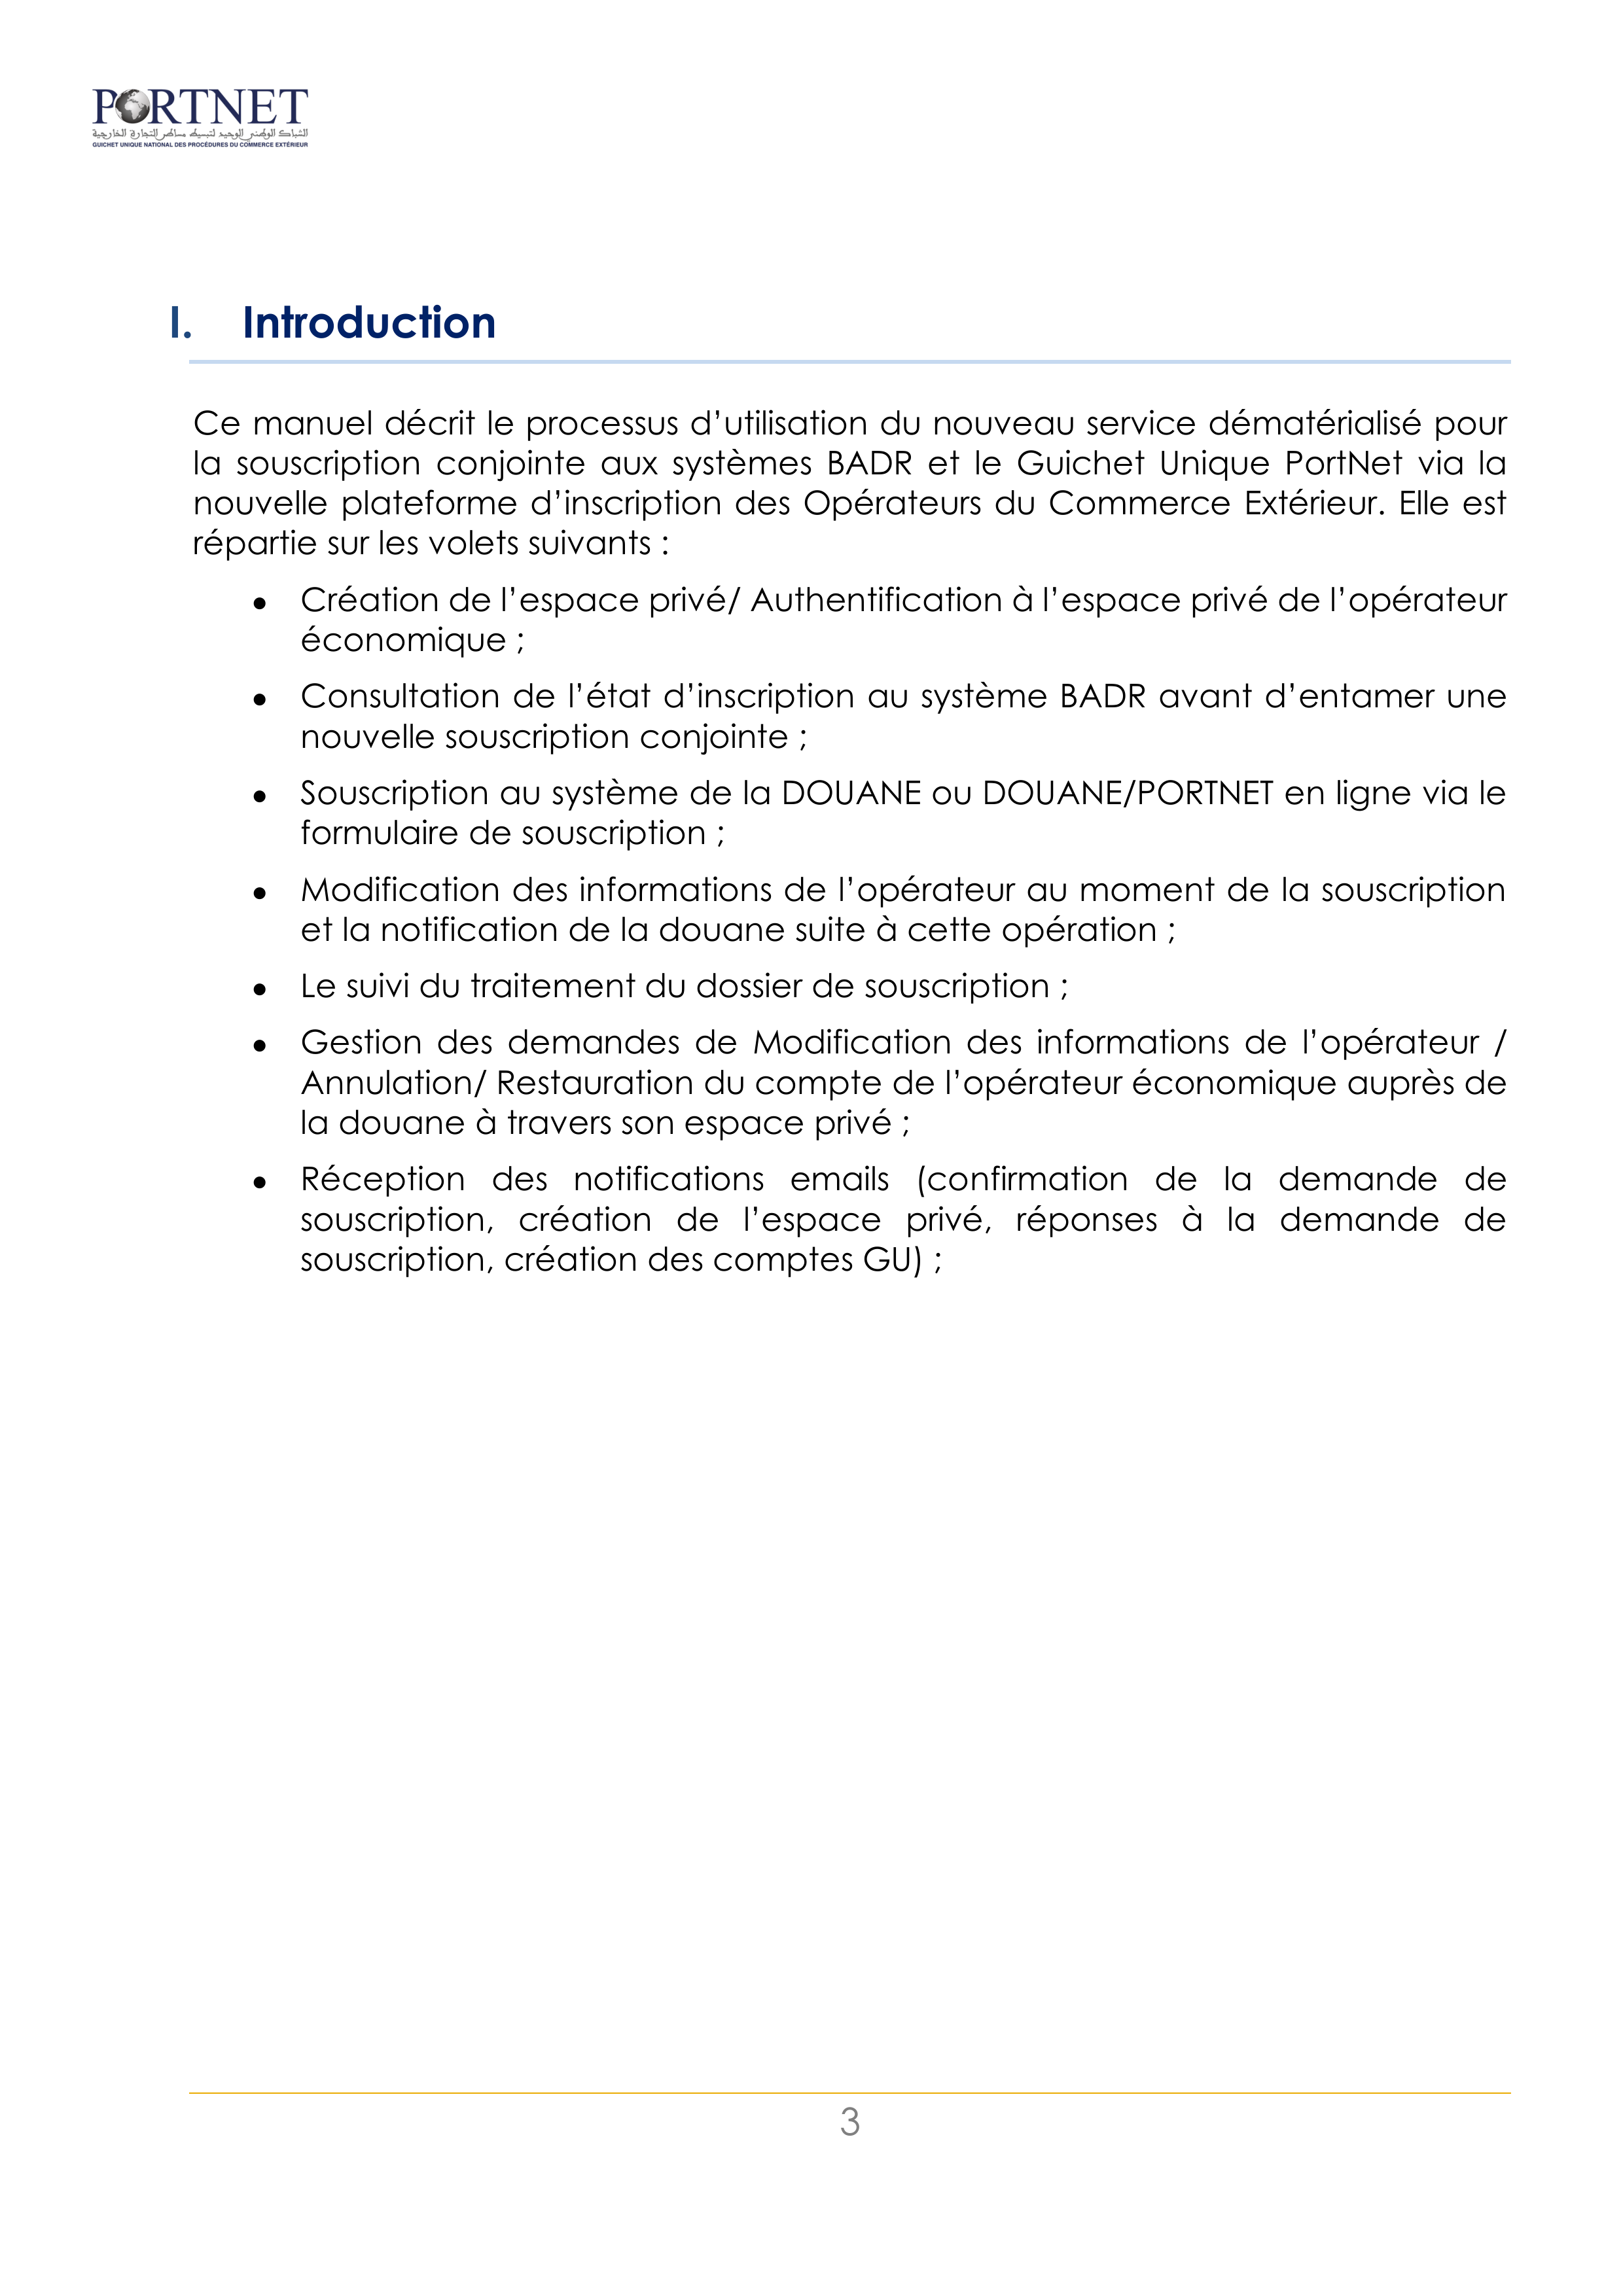
\includegraphics[width=\textwidth]{images/guide_utilisateur_intro.png}
        \caption{Introduction et cadre r\'{e}glementaire du guide officiel.}
        \label{fig:guide-intro}
    \end{minipage}
\end{figure}

\subsection{Critique de l'existant}

Le tableau~\ref{tab:comparaison} présente une analyse comparative entre le système
existant et la solution proposée.

\begin{table}[H]
\centering
\caption{Comparaison entre le système existant et la solution proposée}
\label{tab:comparaison}
\small
\begin{tabular}{|p{3.2cm}|p{4.6cm}|p{4.6cm}|}
\hline
\textbf{Critère} & \textbf{Système existant} & \textbf{Solution proposée} \\
\hline
Identification du type de document & Manuelle, à l'ouverture de chaque fichier &
Classification automatique par ancres textuelles \\
\hline
Lecture des documents numérisés & Lecture visuelle par l'agent &
Reconnaissance optique de caractères (français et arabe) \\
\hline
Validité des identifiants & Non vérifiée &
Contrôle mathématique (modulo 97 du RIB, chiffres de contrôle ICAO de la CNIE) \\
\hline
Cohérence formulaire / documents & Comparaison manuelle, champ par champ &
Rapprochement automatique, avec tolérance sur les libellés \\
\hline
Cohérence entre documents & Non contrôlée systématiquement &
Matrice de cohérence inter-documents \\
\hline
Fraîcheur des documents & Vérifiée au cas par cas &
Contrôle automatique du délai (Modèle J de moins de 90 jours) \\
\hline
Traçabilité & Aucun historique structuré &
Rapport d'audit détaillant chaque contrôle \\
\hline
Temps de traitement & De l'ordre de 15 à 20 minutes par dossier &
Traitement automatisé, contrôle humain limité aux cas douteux \\
\hline
\end{tabular}
\end{table}

\section{Probl\'{e}matique M\'{e}tier et Verrous Techniques}
\subsection{Problématique du projet}
Le mode opératoire actuel présente plusieurs limites structurelles. Le contrôle
d'un dossier complet mobilise un agent pendant une quinzaine à une vingtaine de
minutes, temps qui croît mécaniquement avec le volume de souscriptions. La
comparaison de suites de quinze chiffres (ICE) ou de vingt-quatre caractères
(RIB), répétée des dizaines de fois par jour, est par ailleurs une tâche à fort
risque d'erreur : une inversion de deux chiffres passe aisément inaperçue.

À cela s'ajoute l'impossibilité de détecter la fraude documentaire à l'\oe il nu :
rien ne permet à un agent de savoir qu'un numéro de carte d'identité ou un RIB a
été modifié, alors même que ces identifiants comportent des clés de contrôle
mathématiques exploitables. Un dossier peut également agréger des pièces
appartenant en réalité à deux sociétés distinctes sans que cela soit visible,
faute d'une comparaison systématique champ par champ. Enfin, chaque anomalie
déclenche un aller-retour par courriel qui allonge le délai d'activation du compte
et dégrade l'expérience de l'opérateur.

Dans ce contexte, la question se pose : \textbf{comment automatiser la
vérification des dossiers de souscription, de manière à contrôler systématiquement
l'authenticité des documents et leur cohérence avec les données saisies par
l'opérateur, tout en respectant les contraintes de confidentialité propres à un
tiers de confiance national ?}
\subsection{ Verrous Techniques} 
Le d\'{e}veloppement d'un syst\`{e}me automatique d'inspection documentaire se heurte \`{a} trois verrous techniques majeurs, identifi\'{e}s lors de l'analyse forensique des documents r\'{e}els :

\begin{infobox}
\textbf{Verrou 1 : Faux Positifs Inter-Documents (Cross-Slot Confusion)} \\
Les pi\`{e}ces justificatives marocaines partagent des mentions l\'{e}gales identiques (\texttt{ICE}, \texttt{RC}, \texttt{IF}, \texttt{ROYAUME DU MAROC}). Un algorithme de classification na\"{\i}f bas\'{e} sur la simple pr\'{e}sence de mots-cl\'{e}s acceptait des Mod\`{e}les~J \`{a} la place de la CIN ou de la Taxe Professionnelle. L'analyse forensique a r\'{e}v\'{e}l\'{e} que seule une combinaison d'ancres textuelles exclusives \`{a} chaque type de document permet une discrimination fiable.
\end{infobox}

\begin{infobox}
\textbf{Verrou 2 : Disposition Texte Non-Standard (Value-Before-Label Order)} \\
Les PDF officiels de l'OMPIC et de la DGI placent les valeurs (ex: \texttt{MEDI TELECOM S.A.}) avant ou s\'{e}par\'{e}ment de leurs libell\'{e}s (ex: \texttt{D\'{e}nomination}), pi\'{e}geant les extracteurs traditionnels de type \og label: valeur \fg{}. La solution requiert des strat\'{e}gies d'extraction par zone positionnelle et par ancres contextuelles.
\end{infobox}

\begin{infobox}
\textbf{Verrou 3 : Gestion des Coquilles et Transpositions (Transposition Fallback)} \\
Les fautes de frappe d'un seul caract\`{e}re sur les num\'{e}ros CIN des g\'{e}rants (\texttt{EB21345} vs \texttt{EB12345}) entra\^{\i}naient des rejets stricts non justifi\'{e}s. Le syst\`{e}me doit int\'{e}grer un m\'{e}canisme de tol\'{e}rance bas\'{e} sur la distance d'\'{e}dition de Levenshtein.
\end{infobox}
 
 \section{Objectifs du projet}

Les objectifs assignés au projet sont les suivants :

\begin{enumerate}[leftmargin=1.6cm,itemsep=3pt,topsep=4pt]
  \item \textbf{Classifier automatiquement} les pièces d'un dossier, c'est-à-dire
        reconnaître la nature de chaque fichier déposé sans intervention humaine ;
  \item \textbf{Extraire les données structurantes} de chaque document
        (identifiants, dénominations, adresses, dates), qu'il s'agisse d'un PDF
        natif ou d'un document numérisé nécessitant une reconnaissance optique de
        caractères ;
  \item \textbf{Vérifier la validité intrinsèque} des identifiants officiels au
        moyen de leurs clés de contrôle mathématiques ;
  \item \textbf{Contrôler la cohérence} entre les données du formulaire et celles
        des documents, ainsi qu'entre les documents eux-mêmes ;
  \item \textbf{Produire un rapport d'audit} attribuant à chaque dossier un statut
        exploitable par l'agent --- conforme, à examiner ou non conforme ---
        assorti du détail des contrôles effectués.
\end{enumerate}

Ces objectifs sont encadrés par un ensemble de contraintes imposées par
l'entreprise, résumées dans le tableau~\ref{tab:contraintes}.

\begin{table}[H]
\centering
\caption{Contraintes imposées au projet}
\label{tab:contraintes}
\small
\begin{tabular}{|p{3.2cm}|p{9.2cm}|}
\hline
\textbf{Nature} & \textbf{Contrainte} \\
\hline
Confidentialité & Les documents traités contiennent des données personnelles et
fiscales : aucun recours à un service d'analyse documentaire externe n'est
autorisé, l'intégralité du traitement doit s'exécuter en local. \\
\hline
Matérielle & Le traitement doit fonctionner sur des serveurs standards, sans
accélérateur graphique dédié. \\
\hline
Économique & Recours exclusif à des composants libres, sans coût de licence. \\
\hline
Fonctionnelle & Le système doit tolérer les variations de mise en forme et les
imperfections de numérisation, et ne jamais rejeter un dossier sur la seule foi
d'une lecture automatique incertaine : les cas douteux sont orientés vers un
contrôle humain. \\
\hline
Linguistique & Les documents administratifs marocains sont bilingues
français--arabe et peuvent comporter des chiffres en écriture arabe orientale. \\
\hline
\end{tabular}
\end{table}



\section{Cahier des Charges Fonctionnel et Non-Fonctionnel}

\subsection{Exigences Fonctionnelles}

Le tableau~\ref{tab:exigences-fonctionnelles} r\'{e}capitule les douze exigences fonctionnelles identifi\'{e}es :

\begin{table}[H]
\centering
\small
\begin{tabularx}{\textwidth}{@{}>{\bfseries}p{1.5cm} Y >{\bfseries}p{2cm}@{}}
\toprule
\rowcolor{lightblue}
ID & Description de l'Exigence & Priorit\'{e} \\
\midrule
FR-01 & Proposer une interface web SPA responsive multi-\'{e}tapes (\textit{Wizard}). & Haute \\
FR-02 & G\'{e}rer le mode adaptatif d'inscription (\texttt{DOUANE} ou \texttt{PORTNET\_DOUANE}). & Haute \\
FR-03 & Fournir des emplacements d'upload Drag \& Drop HTML5 par type de document. & Haute \\
FR-04 & Effectuer une v\'{e}rification d'emplacement en temps r\'{e}el (\textit{Realtime Slot Verification}). & Critique \\
FR-05 & Rejeter les faux positifs d'emplacement via un classifier \`{a} 2 couches. & Critique \\
FR-06 & Extraire les entit\'{e}s m\'{e}tier (Raison Sociale, ICE, RC, IF, TP, Adresse, G\'{e}rants, RIB). & Haute \\
FR-07 & Valider la r\'{e}cence du Mod\`{e}le~J selon la r\`{e}gle stricte des 3 mois ($< 90$ jours). & Critique \\
FR-08 & Contr\^{o}ler les cl\'{e}s de v\'{e}rification math\'{e}matique Modulo~97 (ICE et RIB). & Critique \\
FR-09 & Ex\'{e}cuter la Matrice de Coh\'{e}rence Crois\'{e}e (\textit{Cross-Reference Matrix}). & Critique \\
FR-10 & G\'{e}rer la tol\'{e}rance aux fautes de frappe sur les CIN g\'{e}rants (\textit{Transposition Fallback}). & Moyenne \\
FR-11 & G\'{e}n\'{e}rer un rapport de synth\`{e}se interactif avec badges d'\'{e}tat (Vert/Rouge/Orange). & Haute \\
FR-12 & Persister les dossiers valid\'{e}s dans une base relationnelle PostgreSQL. & Haute \\
\bottomrule
\end{tabularx}
\caption{Matrice des exigences fonctionnelles du syst\`{e}me de souscription.}
\label{tab:exigences-fonctionnelles}
\end{table}

\subsection{Exigences Non-Fonctionnelles}

\begin{table}[H]
\centering
\small
\begin{tabularx}{\textwidth}{@{}>{\bfseries}p{1.5cm} Y >{\bfseries}p{2cm}@{}}
\toprule
\rowcolor{lightblue}
ID & Description de l'Exigence & Priorit\'{e} \\
\midrule
NFR-01 & Temps de r\'{e}ponse inf\'{e}rieur \`{a} 3 secondes par document PDF. & Haute \\
NFR-02 & Compatibilit\'{e} navigateur (Chrome, Firefox, Edge, Safari). & Haute \\
NFR-03 & Architecture modulaire et extensible (nouveaux types de documents). & Haute \\
NFR-04 & Code source document\'{e} et test\'{e} (couverture $\geq 90\%$). & Moyenne \\
NFR-05 & S\'{e}curit\'{e} des donn\'{e}es sensibles (CIN, informations fiscales). & Critique \\
NFR-06 & D\'{e}ploiement containeris\'{e} (Docker, uvicorn). & Moyenne \\
\bottomrule
\end{tabularx}
\caption{Matrice des exigences non-fonctionnelles.}
\label{tab:exigences-nfr}
\end{table}

\section{Choix de la Stack Technologique}

Le choix des technologies a \'{e}t\'{e} motiv\'{e} par les crit\`{e}res de performance, de maintenabilit\'{e} et de compatibilit\'{e} avec l'\'{e}cosyst\`{e}me PortNet. Le tableau~\ref{tab:stack-technologique} synth\'{e}tise les choix effectu\'{e}s et les alternatives \'{e}cart\'{e}es :

\begin{table}[H]
\centering
\small
\begin{tabularx}{\textwidth}{@{}>{\bfseries}p{2.5cm} p{3cm} p{3cm} Y@{}}
\toprule
\rowcolor{lightblue}
Composant & Choix retenu & Alternatives & Justification \\
\midrule
Langage backend & Python 3.11 & Java, Node.js & \'{E}cosyst\`{e}me NLP et PDF mature (PyMuPDF, RapidFuzz) \\
Framework API & FastAPI & Django, Flask & Performances async, validation Pydantic native \\
Base de donn\'{e}es & PostgreSQL 15 & MySQL, MongoDB & Transactions ACID, support JSON natif \\
Extraction PDF & PyMuPDF (fitz) & pdfplumber, Tabula & Extraction rapide du texte vectoriel natif \\
Moteur OCR (Tier 2) & Tesseract OCR 5 & Google Vision, Textract & Gratuit, d\'{e}ployable hors-ligne, confidentialit\'{e} \\
Pr\'{e}traitement Image & OpenCV (cv2) & Pillow (PIL), ImageMagick & Binarisation adaptative et deskew pour l'OCR \\
Validation Donn\'{e}es & Pydantic v2 & dataclasses, marshmallow & Validation automatique, mod\'{e}lisation des 7 docs \\
Matching flou & RapidFuzz & FuzzyWuzzy, difflib & 10x plus rapide que FuzzyWuzzy, C++ natif \\
Frontend SPA & HTML/CSS/JS natif & React, Angular & Simplicit\'{e}, z\'{e}ro d\'{e}pendance, portail PortNet \\
Framework Tests & pytest 7.x & unittest, nose2 & Fixtures flexibles, validation 64 cas (100\% PASS) \\
Containerisation & Docker \& Compose & Machines Virtuelles (VM) & Isolation environnement, d\'{e}ploiement reproductible \\
\bottomrule
\end{tabularx}
\caption{Tableau comparatif de la stack technologique (11 composants).}
\label{tab:stack-technologique}
\end{table}

\begin{figure}[H]
    \centering
    \IfFileExists{images/comparaison_stack.png}{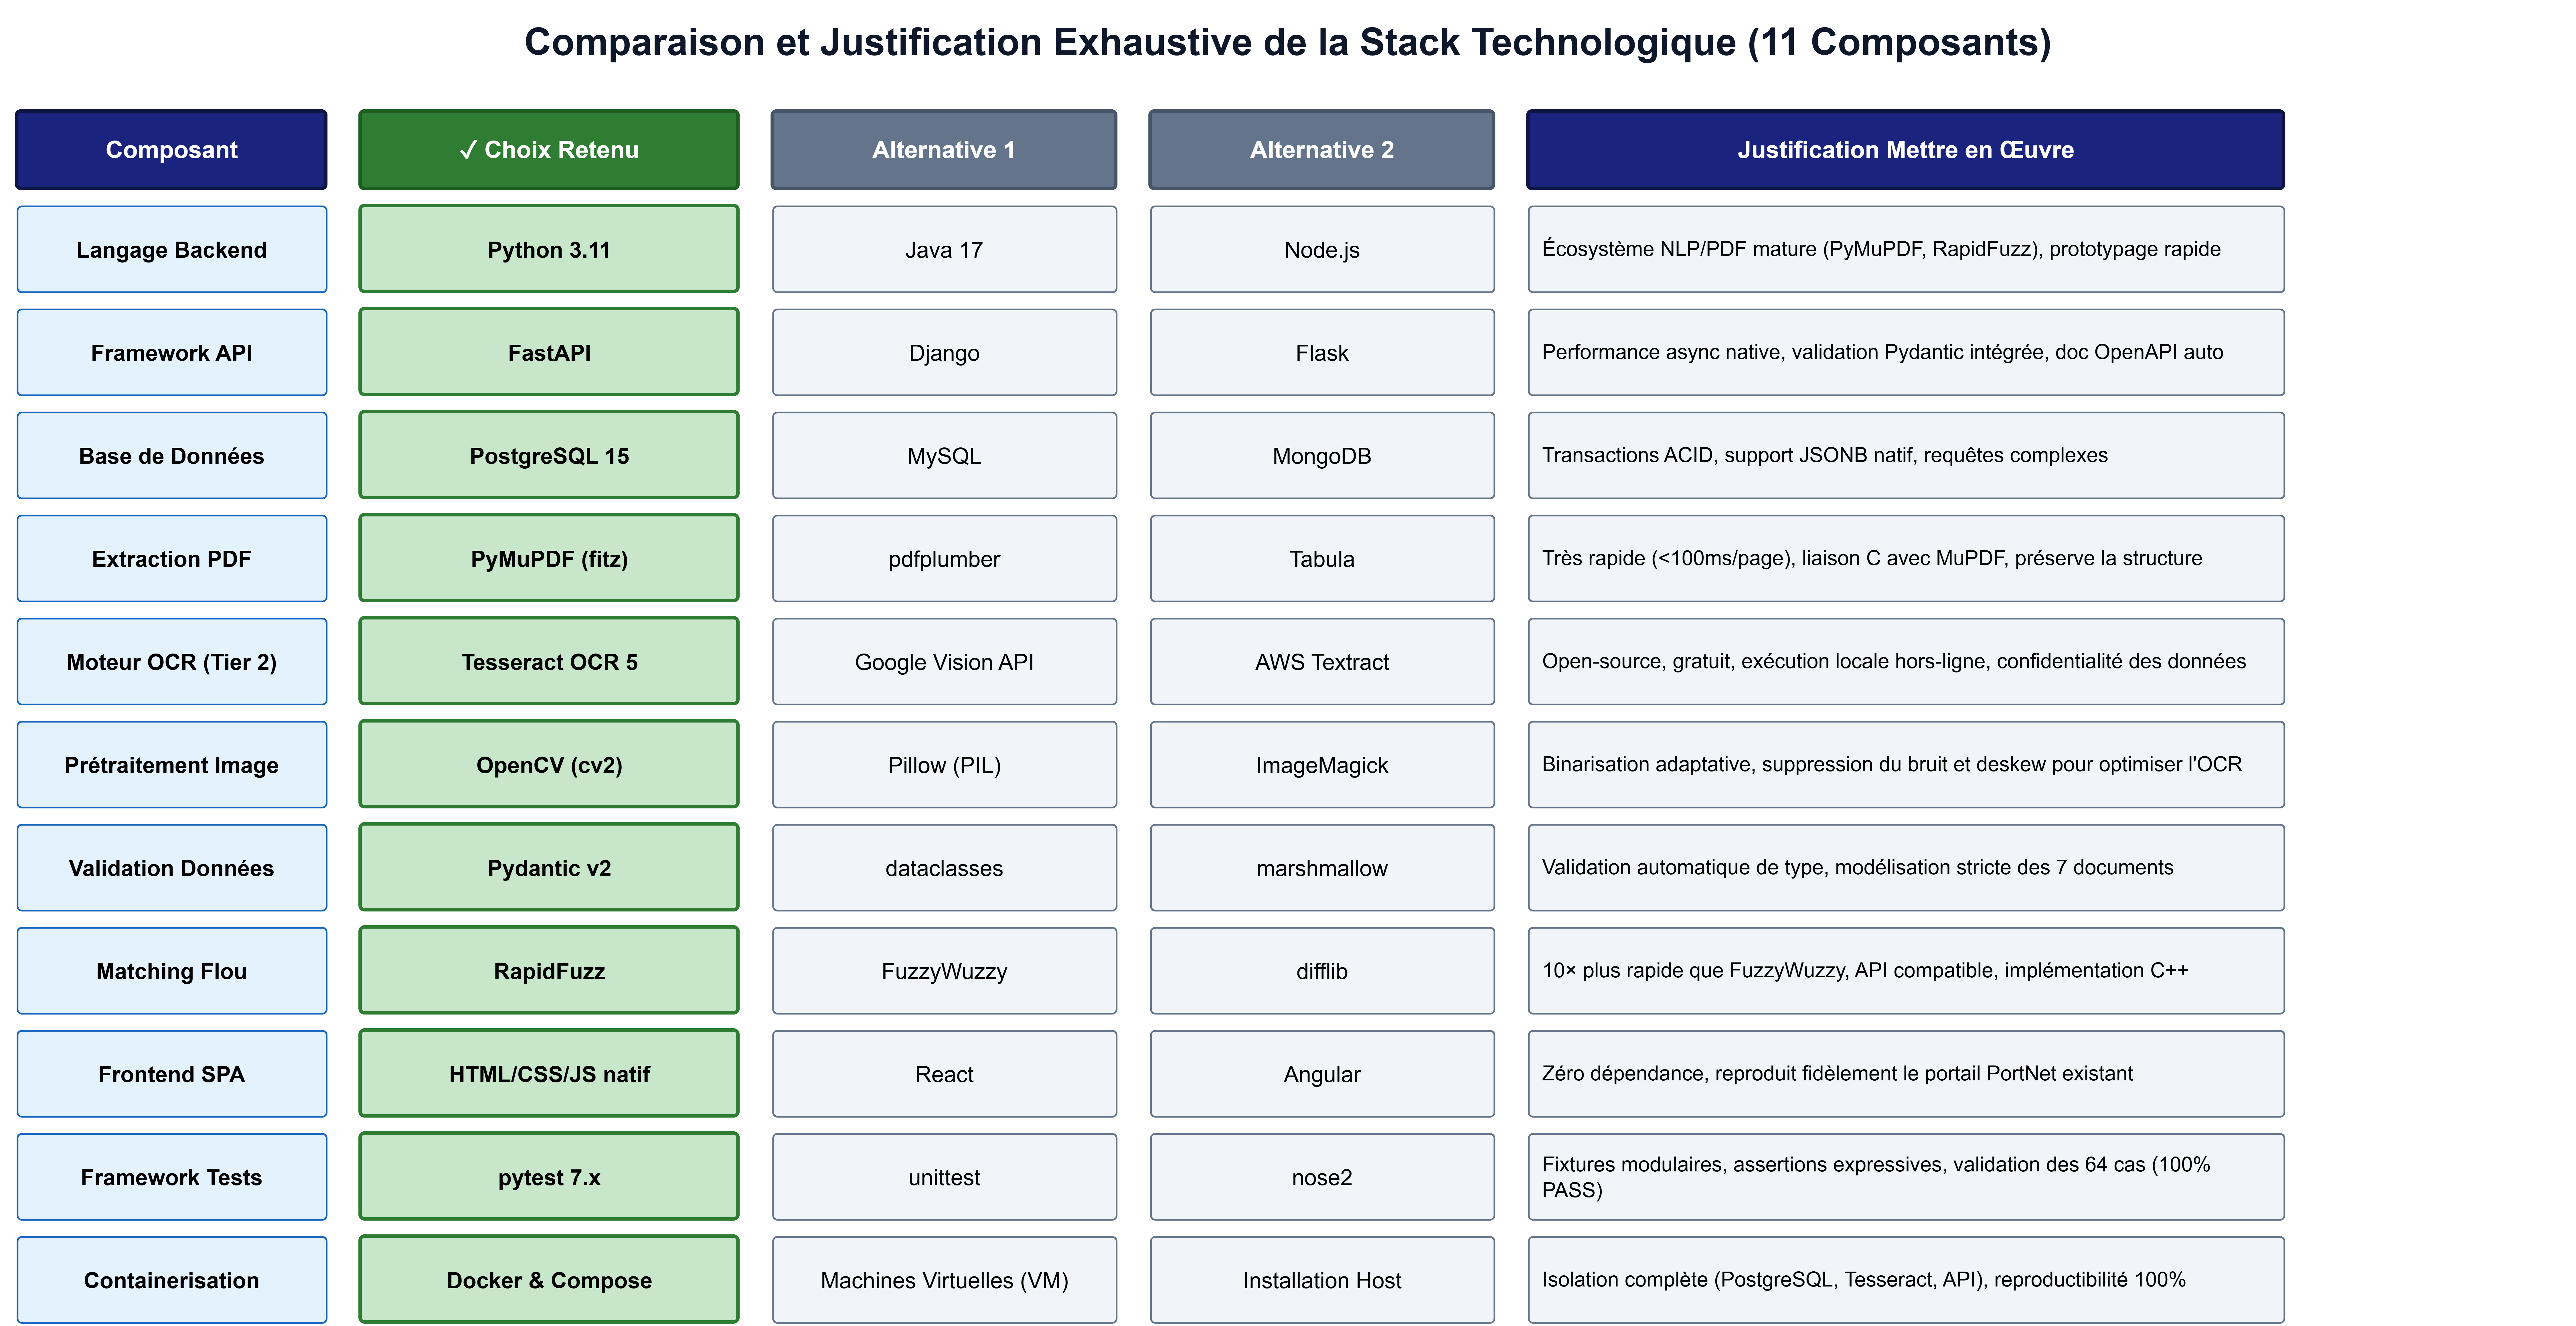
\includegraphics[width=\textwidth]{images/comparaison_stack.png}}{\fbox{\parbox{14cm}{\centering\vspace{1.5cm}\textit{Comparaison visuelle de la stack --- Exporter depuis comparaison\_stack.drawio}\vspace{1.5cm}}}}
    \caption{Comparaison visuelle des technologies retenues et alternatives \'{e}cart\'{e}es.}
    \label{fig:comparaison-stack}
\end{figure}

\begin{figure}[H]
    \centering
    \small
    \begin{tabular}{c c c c}
        
\includegraphics[height=1.1cm]{Logos/logo_python.png} &
        
\includegraphics[height=1.1cm]{Logos/logo_fastapi.png} &
        
\includegraphics[height=1.1cm]{Logos/logo_postgresql.png} &
        
\includegraphics[height=1.1cm]{Logos/logo_docker.png} \\[0.3cm]
        \textbf{Python 3.11} & \textbf{FastAPI} & \textbf{PostgreSQL} & \textbf{Docker} \\[0.5cm]
        
        
\includegraphics[height=1.1cm]{Logos/logo_pymupdf.png} &
        
\includegraphics[height=1.1cm]{Logos/logo_tesseract.png} &
        
\includegraphics[height=1.1cm]{Logos/logo_opencv.png} &
        
\includegraphics[height=1.1cm]{Logos/logo_pydantic.png} \\[0.3cm]
        \textbf{PyMuPDF} & \textbf{Tesseract OCR} & \textbf{OpenCV} & \textbf{Pydantic} \\[0.5cm]

        
\includegraphics[height=1.1cm]{Logos/logo_html5.png} &
        
\includegraphics[height=1.1cm]{Logos/logo_css3.png} &
        
\includegraphics[height=1.1cm]{Logos/logo_javascript.png} &
        
\includegraphics[height=1.1cm]{Logos/logo_pytest.png} \\[0.3cm]
        \textbf{HTML5} & \textbf{CSS3} & \textbf{JavaScript} & \textbf{pytest} \\
    \end{tabular}
    \caption{Panorama des technologies et composantes logicielles de la solution.}
    \label{fig:tech-stack-logos}
\end{figure}

\section{Planning du projet}

Le projet s'est déroulé sur neuf semaines, du 15 juin au 15 août 2026, selon une
démarche itérative et incrémentale rythmée par des points d'avancement
hebdomadaires avec l'encadrement de l'entreprise. Chaque itération livrait une
brique fonctionnelle validée par une démonstration sur des documents réels.

\begin{table}[H]
\centering
\caption{Déroulement du stage}
\label{tab:planning}
\small
\begin{tabular}{|p{1.8cm}|p{3.8cm}|p{6.6cm}|}
\hline
\textbf{Semaines} & \textbf{Phase} & \textbf{Travaux réalisés} \\
\hline
S1--S2 & Intégration et cadrage &
Découverte de PortNet et de son écosystème, étude du besoin, mise en place de
l'environnement de développement. \\
\hline
S3--S4 & Étude préliminaire &
Modélisation et alimentation de la base de données, analyse du processus de
souscription et du corpus documentaire. \\
\hline
S5 & Conception &
Étude comparative des moteurs de reconnaissance optique de caractères, conception
de la chaîne de traitement et de la matrice de cohérence. \\
\hline
S6--S7 & Réalisation &
Développement du prétraitement d'image et de l'OCR, des analyseurs de documents,
des contrôles mathématiques et du moteur de rapprochement. \\
\hline
S8 & Extension et intégration &
Formulaire de souscription, interface applicative d'enregistrement, base de
données, intégration des contributions du binôme. \\
\hline
S9 & Tests et restitution &
Campagne de tests sur documents réels, démonstrations, rédaction du rapport. \\
\hline
\end{tabular}
\end{table}

Le projet ayant été mené en binôme, le partage des développements s'est fait selon
la nature des documents et des briques techniques : la chaîne de traitement et la
matrice de cohérence ont été conçues conjointement, tandis que j'ai pris en charge
le traitement des documents \textbf{numérisés} (prétraitement d'image,
reconnaissance optique de caractères, lecture et validation de la carte nationale
d'identité électronique, formulaire et base de données) et que mon binôme a traité
les documents \textbf{nativement numériques} (extraction de texte vectoriel,
analyseurs par type de document, moteur de rapprochement).

\section*{Conclusion du Chapitre}

Ce premier chapitre a permis de situer le projet dans son contexte institutionnel et m\'{e}tier. L'analyse critique du processus existant a mis en \'{e}vidence des faiblesses structurelles justifiant le d\'{e}veloppement d'un syst\`{e}me automatis\'{e} de v\'{e}rification documentaire. La formalisation du cahier des charges et le choix de la stack technologique \'{e}tablissent les fondations sur lesquelles s'appuieront les chapitres suivants. Le Chapitre~2 pr\'{e}sentera l'\'{e}tat de l'art des techniques d'extraction, de classification et de validation documentaire.
